\section{评测}

我们首先用多种智能体 RL 任务评估 \sysname 的 ACT 效率（\S\ref{sec:e2e}），随后考察其随 RL batch size 与外部资源规模变化时的可扩展性（\S\ref{sec:eval_scale}），最后分析 \sysname 的设计效果与系统开销（\S\ref{sec:eval_analyse}）。

\begin{figure*}[t]
    \begin{minipage}{0.24\linewidth}
        \centerline{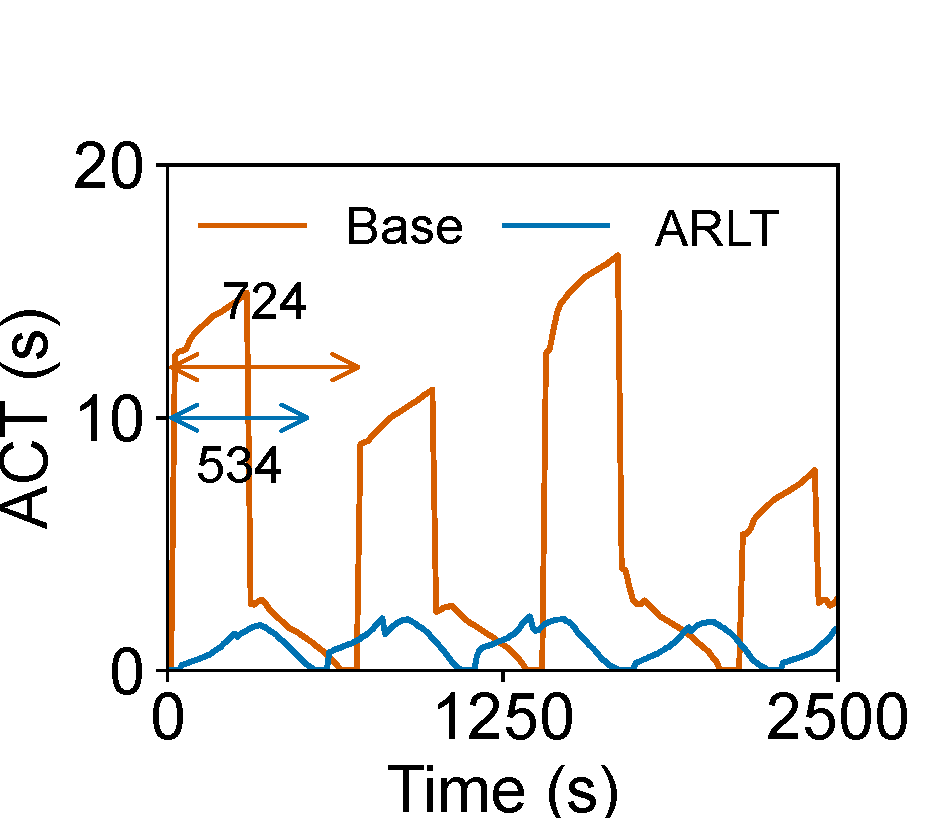
\includegraphics[width=\linewidth,trim=0 0 0 20,clip]{figures/Eval_e2e_act_code.pdf}}
        \centerline{\small (a) AI Coding.}
        \vspace{-0.1in}
    \end{minipage}
    \begin{minipage}{0.24\linewidth}
        \centerline{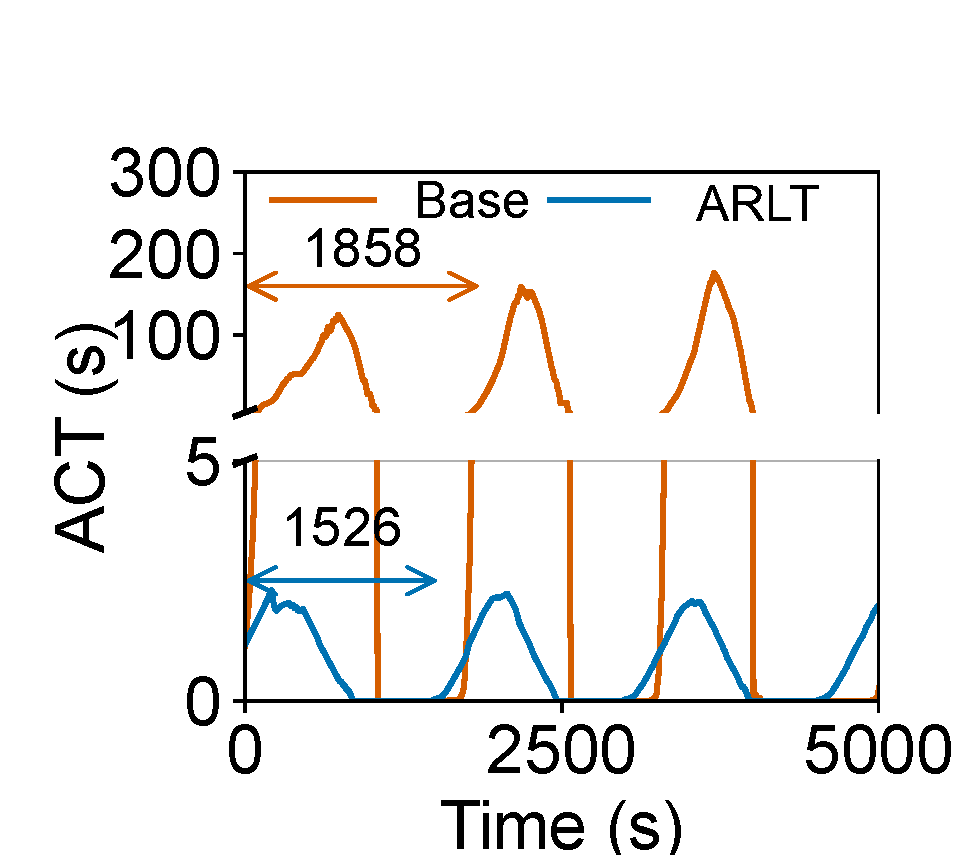
\includegraphics[width=\linewidth,trim=0 0 0 20,clip]{figures/Eval_e2e_act_mopd.pdf}}
        \centerline{\small (b) MOPD.}
        \vspace{-0.1in}
    \end{minipage}
    \begin{minipage}{0.24\linewidth}
        \centerline{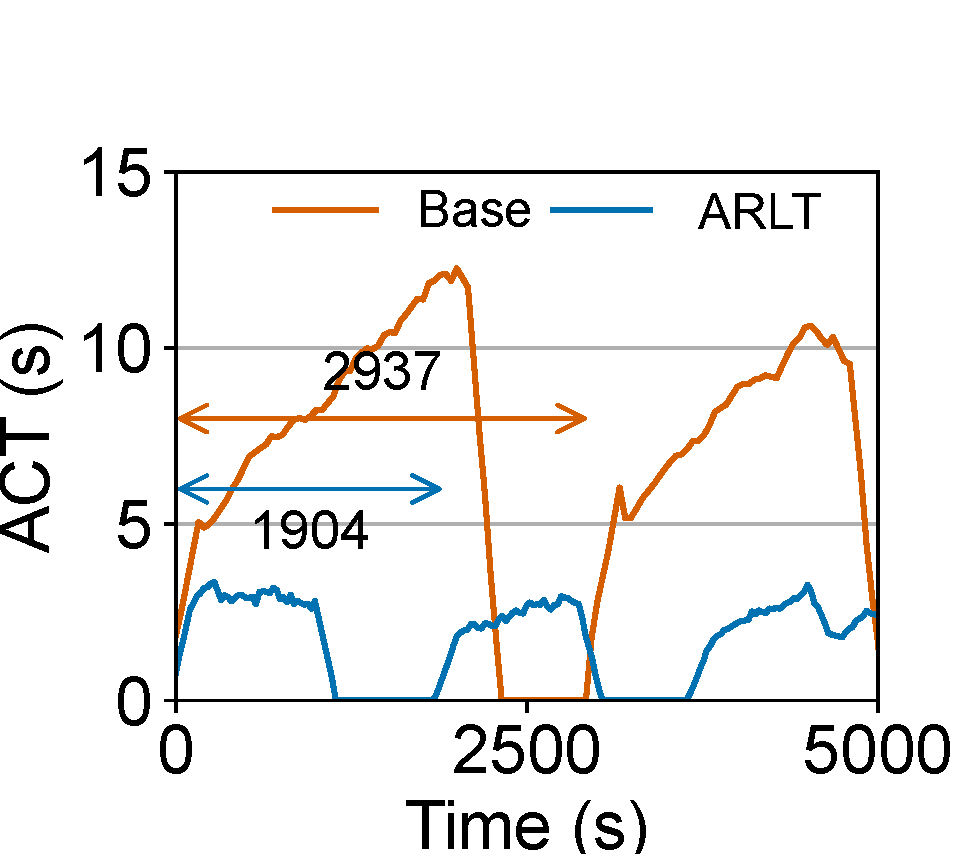
\includegraphics[width=\linewidth,trim=0 0 0 20,clip]{figures/Eval_e2e_act_search.pdf}}
        \centerline{\small (c) DeepSearch.}
        \vspace{-0.1in}
    \end{minipage}
    \begin{minipage}{0.24\linewidth}
        \centerline{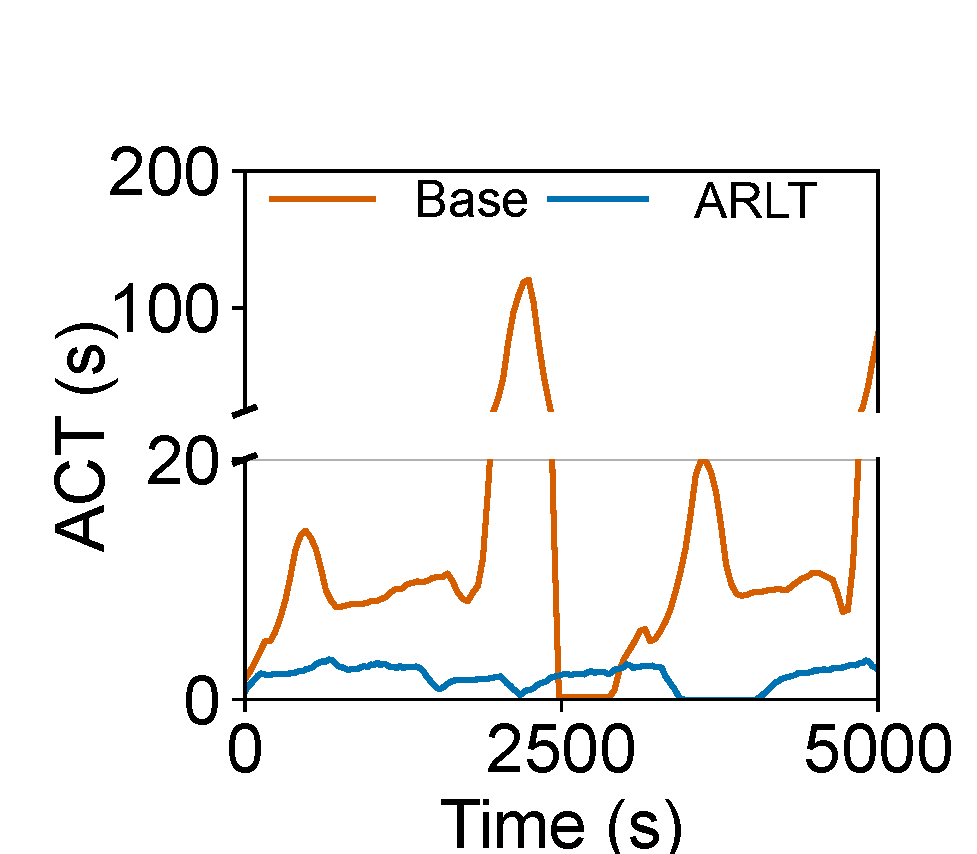
\includegraphics[width=\linewidth,trim=0 0 0 20,clip]{figures/Eval_e2e_act_sm.pdf}}
        \centerline{\small (d) MOPD+DeepSearch.}
        \vspace{-0.1in}
    \end{minipage}
    \caption{不同 RL 任务下的 ACT。图中数字和箭头表示 RL 任务的 step 时长。}
    \label{fig:eval_specific_lat}
    \vspace{-0.15in}
\end{figure*}

\subsection{实验设置}
\label{sec:setup}
\paraf{测试平台。} 测试平台由两部分组成：一部分是运行智能体 RL 框架的 GPU 集群，另一部分是由 \sysname 管理的一组异构外部资源。RL 框架部署在生产环境 GPU 集群上，最多包含 48 个 GPU 节点，每个节点配备 8 张基于 NVIDIA Hopper 架构的 GPU，并通过高带宽 NVLink 与 RDMA 网络互联。我们使用 VeRL~\citep{sheng2025hybridflow} 作为智能体 RL 框架，并为其扩展了外部资源调用、序列级和异步 \textit{rollout} 能力。\sysname 同时部署在 CPU 与 GPU 集群上：CPU 集群包含 15 个节点，每个节点拥有 256 个 AMD CPU 核和 2.4 TB 内存；GPU 集群包含 5 个节点，每个节点拥有 8 张高端 NVIDIA GPU 和 3 TB CPU 内存。此外，\sysname 还管理若干带配额限制的外部 API 服务，例如 Google Search 和 PDF 解析服务。

\parabf{工作负载。} 我们在 \S\ref{sec:e2e} 中选取三类智能体 RL 任务作为工作负载。 \textbf{AI Coding} 使用 CPU 构建隔离执行环境，环境会被间歇性调用，并用于计算奖励分数。我们采用一个面向生产环境、基于 SWEBench~\citep{jimenez2024swebench} 脚手架构造的内部数据集。 \textbf{DeepSearch} 持续访问外部网站来辅助 LLM 问答，其数据集基于 BrowseComp~\citep{wei2025browsecomp}，奖励则由基于 LLM 的判别器在生成轨迹上进行计算，具体使用微调后的 GPT-OSS~\citep{agarwal2025gpt}。上述两个任务都采用 GRPO~\citep{shao2024deepseekmath}。 \textbf{MOPD}~\citep{xiao2026mimo} 在 rollout 阶段同时整合多个 RL 任务（包括智能体任务），并相对于对应教师模型计算轨迹对数概率以完成对齐。为了展示 \sysname 在缓解“RL 任务内部过量预留”方面的收益，我们还让 DeepSearch 与 MOPD 并发运行，因为二者都需要 GPU 来部署外部服务。

\parabf{基线。}
由于没有现有系统能统一支持这三类工作负载，我们为 \S\ref{sec:e2e} 中的实验分别设计了任务特定基线。对于 \textbf{AI Coding}，我们使用 Kubernetes 管理 CPU 集群。每条轨迹在执行开始时申请创建一个 pod，每个 pod 分配 0.5 个 CPU，以允许有限复用，同时设定最多 4 个 CPU 的上限以避免拥塞。对于 \textbf{MOPD}，我们使用 SGLang~\citep{zheng2024sglang} 在 GPU 集群上部署 9 个教师模型，每个模型分配 4 张 GPU 并使用 tensor parallelism（TP）。对于 \textbf{DeepSearch}，基线允许每条轨迹独立执行 API 调用，并在错误时最多重试 3 次，超时阈值为 600 秒。DeepSearch 的奖励服务也部署在 GPU 集群上，共 5 个副本，TP 度数为 8。对于“MOPD+Search”，共部署 10 个奖励服务，每个模型分配 4 张 GPU 且采用 TP。

\parabf{指标。}
为了比较 \sysname 与基线的效率，我们主要测量平均 ACT。同时，我们还报告多个阶段的细粒度时长，包括 LLM 生成、工具调用和奖励计算。所有阶段时长都用 \sysname 的总时长归一化，因此 \sysname 的归一化时长总和为 1。

\parabf{其他设置。}
本节中，不同工作负载的 RL 训练 batch size 与外部资源容量固定为：AI Coding 为 1280，MOPD 为 2048，DeepSearch 为 2048。RL 训练模型使用 Qwen3-32B~\citep{yang2025qwen3} 与 MiMo-V2-Flash~\citep{xiao2026mimo}。此外，\sysname 的具体配置包括：调度算法中的 $depth$ 设为 2；只对 CPU 上的奖励计算和 GPU 上的奖励模型推理预先做可扩展性与执行时长 profiling。

\subsection{端到端性能}
\label{sec:e2e}

\begin{figure}[t]
    \centerline{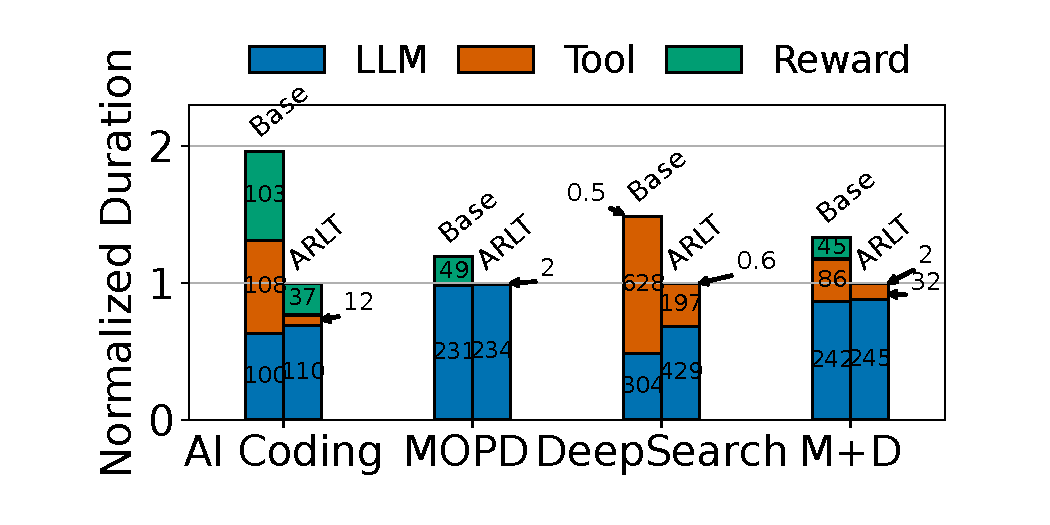
\includegraphics[width=0.6\linewidth]{figures/Eval_e2e.pdf}}
    \vspace{-0.3in}
    \caption{不同 RL 任务上的端到端性能。柱状图中的数字表示绝对时长（秒）。}
    \label{fig:eval_e2e}
    \vspace{-0.25in}
\end{figure}

我们在多种工作负载上评估端到端性能，以展示 \sysname 的通用性与效率。图~\ref{fig:eval_specific_lat} 给出了 RL 训练推进过程中、连续小时间窗口内的平均 ACT。可以看到，在所有工作负载下，\sysname 的 ACT 都持续低于基线。这说明在给定相同外部资源条件下，\sysname 能更有效地处理突发工作负载，并通过缓解过量预留、提高外部资源利用率来降低 ACT。即便 DeepSearch 中的 API 调用本身不可扩展，对配额和并发的合理管理也能减少由于限流或超时引起的错误和重试，从而降低 ACT。

我们进一步报告了 10 个 RL 训练 step 的平均时长，即 \textbf{step duration}，以体现 \sysname 对端到端训练效率的提升。AI Coding 和 DeepSearch 的 step 时长分别获得了 $1.4\times$ 和 $1.5\times$ 的显著优化。对 AI Coding 而言，收益主要来自动作级调度，它提高了外部 CPU 的利用率；对 DeepSearch 而言，由于 API 调用本身不可扩展，step 时长的下降主要来自流量控制与更稳定的调用行为。总体上，\sysname 通过缩短外部调用等待时间和提升资源复用效率，提高了训练系统的端到端效率。

\subsection{系统可扩展性}
\label{sec:eval_scale}

\begin{figure}[t]
    \begin{minipage}{0.48\linewidth}
    \centerline{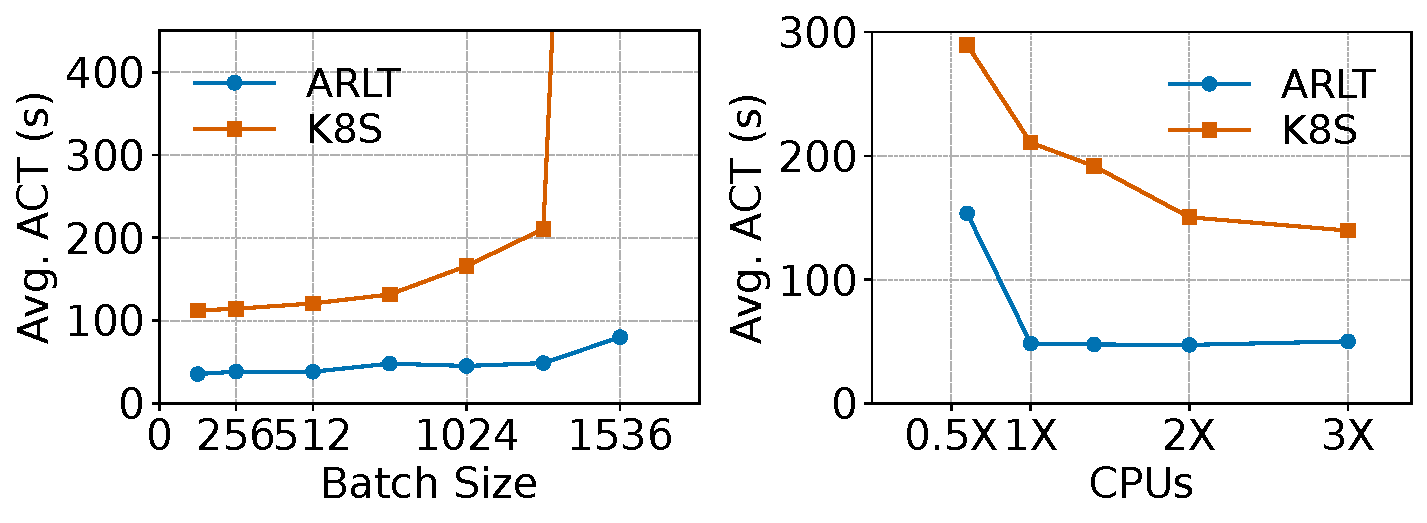
\includegraphics[width=\linewidth]{figures/Eval_cpu_scale.pdf}}
    \centerline{\small (a) CPU 的可扩展性。}
    \end{minipage}
    \begin{minipage}{0.48\linewidth}
    \centerline{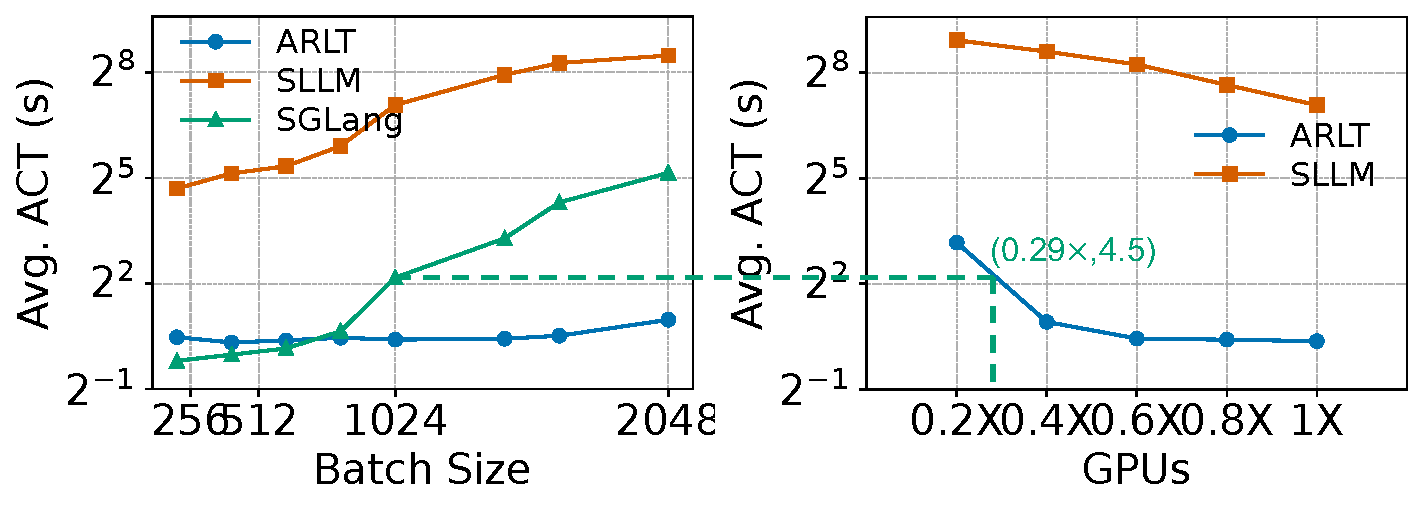
\includegraphics[width=\linewidth]{figures/Eval_gpu_scale_new.pdf}}
    \centerline{\small (b) GPU 的可扩展性。}
    \end{minipage}
    \caption{不同外部资源在 RL batch size 和资源容量变化下的可扩展性。}
    \label{fig:eval_scale}
\end{figure}

我们进一步通过同时放大并发度和资源容量来评估 \sysname 的有效性。重点考察那些动作本身可扩展的资源，也就是 CPU 和 GPU。我们测量每条轨迹的总 ACT，并在不同 \textbf{batch size} 和 \textbf{资源容量} 下取轨迹平均。由于采用 GRPO，因此每个 batch 中的轨迹数可以视作 RL batch size。

\parabf{CPU 的可扩展性。}
在图~\ref{fig:eval_scale}(a) 中，所有实验都使用 5 个节点共 1280 个 CPU 核作为外部资源。随着 RL batch size 增大，\sysname 相比基线可将平均 ACT 降低 $3.1\times$ 到 $27.7\times$。尤其在 batch size 为 1536 时，Kubernetes 基线由于资源不足，其控制平面开始频繁出现排队超时；而 \sysname 在该规模下仍能保持可接受的 ACT 增长，相比 batch size 为 128 时的 ACT 增幅不足 $2\times$。右图固定 batch size 为 1280，在这一配置下基线仍比 \sysname 慢 $1.89\times$ 到 $4.33\times$。当总 CPU 核数降为 768 时，收益有所减弱，因为资源更少会减少动作级调度跨轨迹复用的空间。

\parabf{GPU 的可扩展性。}
除 SGLang 基线外，我们还引入了 ServerlessLLM~\citep{fu2024serverlessllm} 作为另一个基线，它通过 Model-as-a-Service（MaaS）抽象用更少 GPU 服务多个模型。与 CPU 场景类似，图~\ref{fig:eval_scale}(b) 左侧的实验都在 \S\ref{sec:setup} 所述的 5 节点 GPU 集群上完成。在高 batch size 下，\sysname 显著优于两个基线：当 batch size 为 2048 时，\sysname 相比 SGLang 可将平均 ACT 降低 $18.1\times$，而 ServerlessLLM 在这种并发度下已无法提供可接受服务。作为参考，在 batch size 为 1024 时，\sysname 相比 SGLang 和 ServerlessLLM 分别快 $3.4\times$ 与 $101.8\times$。需要指出的是，在低并发下，由于 \sysname 存在恢复开销，SGLang 的时延会略优一些。

图~\ref{fig:eval_scale}(b) 右侧则进一步说明，在固定 batch size 为 1024 的情况下，\sysname 在降低外部资源成本方面同样具有优势。\sysname 仅使用过量预留基线所需 GPU 数量的 29\%，就能为 10 个奖励服务提供支持并实现相同的 ACT。虽然 \sysname 和 ServerlessLLM 都能用更少 GPU 部署多个模型，但由于 ServerlessLLM 缺少针对奖励服务的弹性重分配机制，且系统开销更高，因此其时延明显更差。

\subsection{\sysname 设计分析}
\label{sec:eval_analyse}
\paraf{\sysname 调度策略的影响。}
我们在 AI Coding 工作负载上对弹性调度算法做了消融分析。由于 CPU 计算负载高度依赖 LLM 输出，随机性较强，我们基于一条真实 AI Coding RL 轨迹构建了一个 benchmark，并据此比较不同调度基线。在该任务中，只有奖励计算类动作具备 CPU 级可扩展性，因为它们执行时间长尾明显，也适合并行化。我们将动态 DoP 在 1 到 32 范围内变化的弹性调度算法，与两个固定 DoP 基线（DoP=4 与 DoP=16）进行比较。图~\ref{fig:eval_scheduling} 表明，弹性调度在所有设置下都优于固定 DoP 基线。其原因在于，它能根据资源竞争情况动态调整资源分配策略。

\begin{figure}[t]
    \centerline{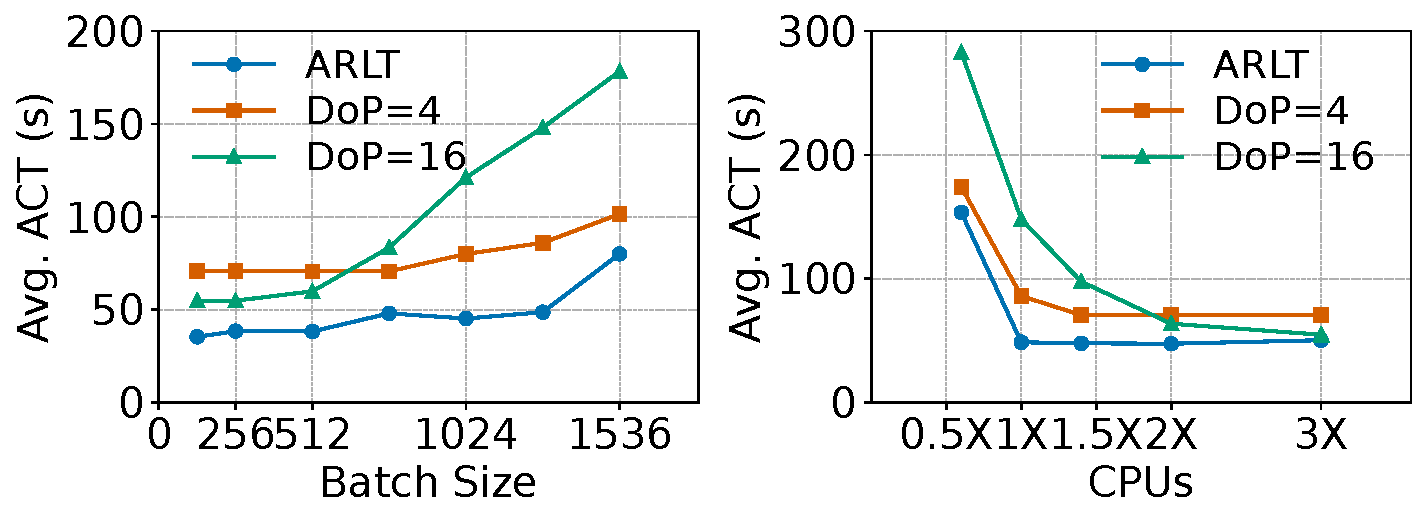
\includegraphics[width=0.6\linewidth]{figures/Eval_schedule.pdf}}
    \caption{\sysname 调度策略的影响。}
    \label{fig:eval_scheduling}
\end{figure}

\parabf{系统开销分析。}
我们进一步分解 AI Coding（CPU 密集）和 MOPD（GPU 密集）的 ACT，以分析系统开销，结果见表~\ref{table:overhead}。可以看到，即便在 AI Coding 的高拥塞场景下，系统开销相对于执行时长仍然只占很小部分；而对 GPU 场景中的 MOPD 而言，恢复带来的额外开销更明显，但这种开销不会随着更高并发或更严重排队而爆炸式增长，因此系统在高并发智能体 RL 训练下仍然能保持稳定与高效。

\begin{table}[!t]
\centering
\begin{tabular}{c|cccc}
\toprule
\makecell[c]{\textbf{工作负载} \\ (bsz)} &
\makecell[c]{\textbf{Coding} \\ (1280)} &
\makecell[c]{\textbf{Coding} \\ (1536)} &
\makecell[c]{\textbf{MOPD} \\ (2048)} &
\makecell[c]{\textbf{MOPD} \\ (3072)} \\
\midrule
执行时长                & 0.975 & 1.206 & 0.621 & 0.705 \\
排队时长               & 0.015 & 0.428 & 0.081 & 15.05 \\
系统开销            & 0.024 & 0.036 & 0.201 & 0.240 \\
\bottomrule
\end{tabular}
\caption{ACT 分解。}
\label{table:overhead}
\vspace{-0.2in}
\end{table}

\parabf{建模精度。}
除了端到端收益，我们还验证了 \sysname 建模的准确性。总体上，执行时长与弹性建模为调度器提供了足够准确的相对比较依据，使其能够在真实系统状态下做出有效的资源分配决策。
